\section{Representation-Based Compression: MRCZ}\label{sec:mrcz}

In this section, we first analyze the compressor introduced in Section~\ref{sec:related work:prior work} in detail. Building on this foundation, we progressively analyze and optimize its design, and ultimately develop a new model-representation-based compressor, MRCZ.

\subsection{Revisiting DLT for HOHS Data Compression}

In Section~\ref{sec:related work:prior work}, we introduced a compressor~\cite{marin2016spectral} for HOHS data generated by Nek5000, which applies discrete Legendre transforms (DLT) on elements defined on GLL nodes. A key observation motivating this approach is that the transformed coefficients tend to be significantly more concentrated than the original data values.
To verify this, we take the 5th NekRS~\cite{fischer2022nekrs} dataset in Table~\ref{tab:datasets} and report the value-frequency distribution.

\begin{figure}[htb]
    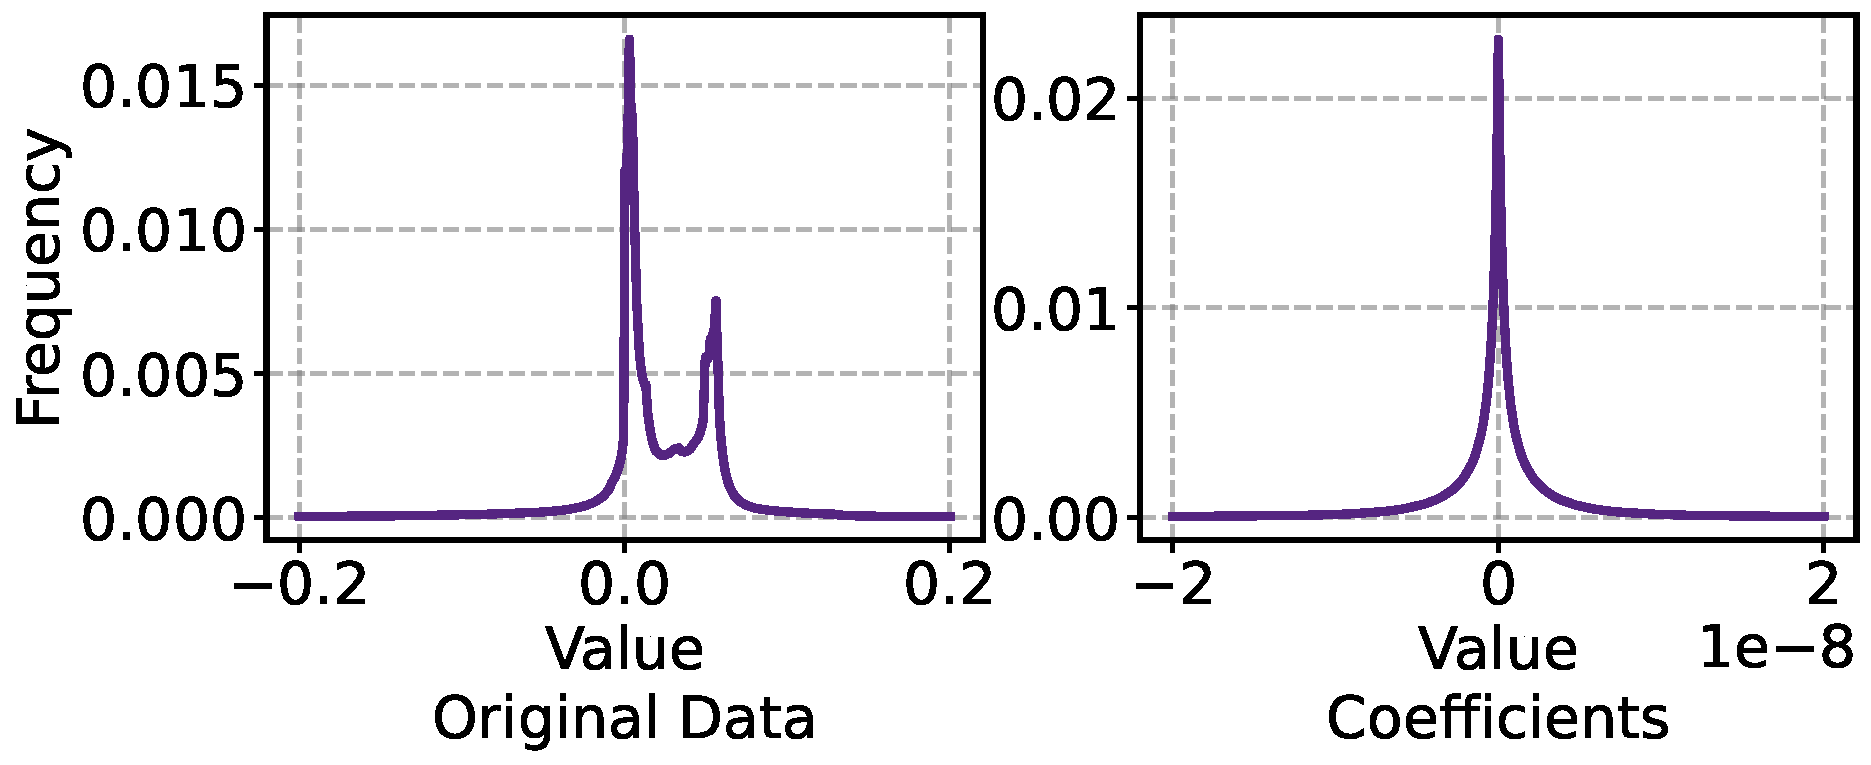
\includegraphics[width=0.8\linewidth]{figs/4-distribution-of-data-and-coefficients.pdf}
    \caption{Distributions of Original Data and Coefficients}
    \label{fig:dlt_distributions}
\end{figure}

Figure~\ref{fig:dlt_distributions} compares the distributions of the original data and the coefficients obtained by applying the DLT to HOHS data defined on GLL nodes. In this example, most coefficients are confined to a range approximately $10^{-7}$ times as wide as the range containing most of the original data. This strong concentration benefits the thresholding strategy used in the previously mentioned method~\cite{marin2016spectral}, which sets sufficiently small coefficients to zero. A more concentrated coefficient distribution, therefore, allows a larger fraction of coefficients to be zeroed, thereby reducing the storage footprint. Moreover, because the Legendre basis is orthogonal under the GLL quadrature-weighted inner product, errors introduced by coefficient thresholding are not strongly amplified during the inverse transform. Thus, discarding coefficients of sufficiently small magnitude generally leads to limited reconstruction error.

However, the reconstruction error introduced by the previously discussed thresholding method is only indirectly controlled and does not necessarily satisfy a user-specified pointwise error bound. In contrast, as described in Section~\ref{sec:design overview:family}, the SZ framework enforces the prescribed error bound independently of the specific prediction strategy, whether it is interpolation-based or transform-based. Therefore, strict orthogonality of the transform is not essential for error control. As long as the transform is invertible and numerically stable, its primary role is to produce coefficients that are more compressible. This observation decouples compression effectiveness from the mathematical properties of the DLT and suggests that alternative transforms, if better aligned with the data structure, may achieve stronger coefficient compaction. This motivates us to explore transformation choices beyond the DLT.

\subsection{Overview of MRCZ}

\begin{figure}[htb]
    \centering
    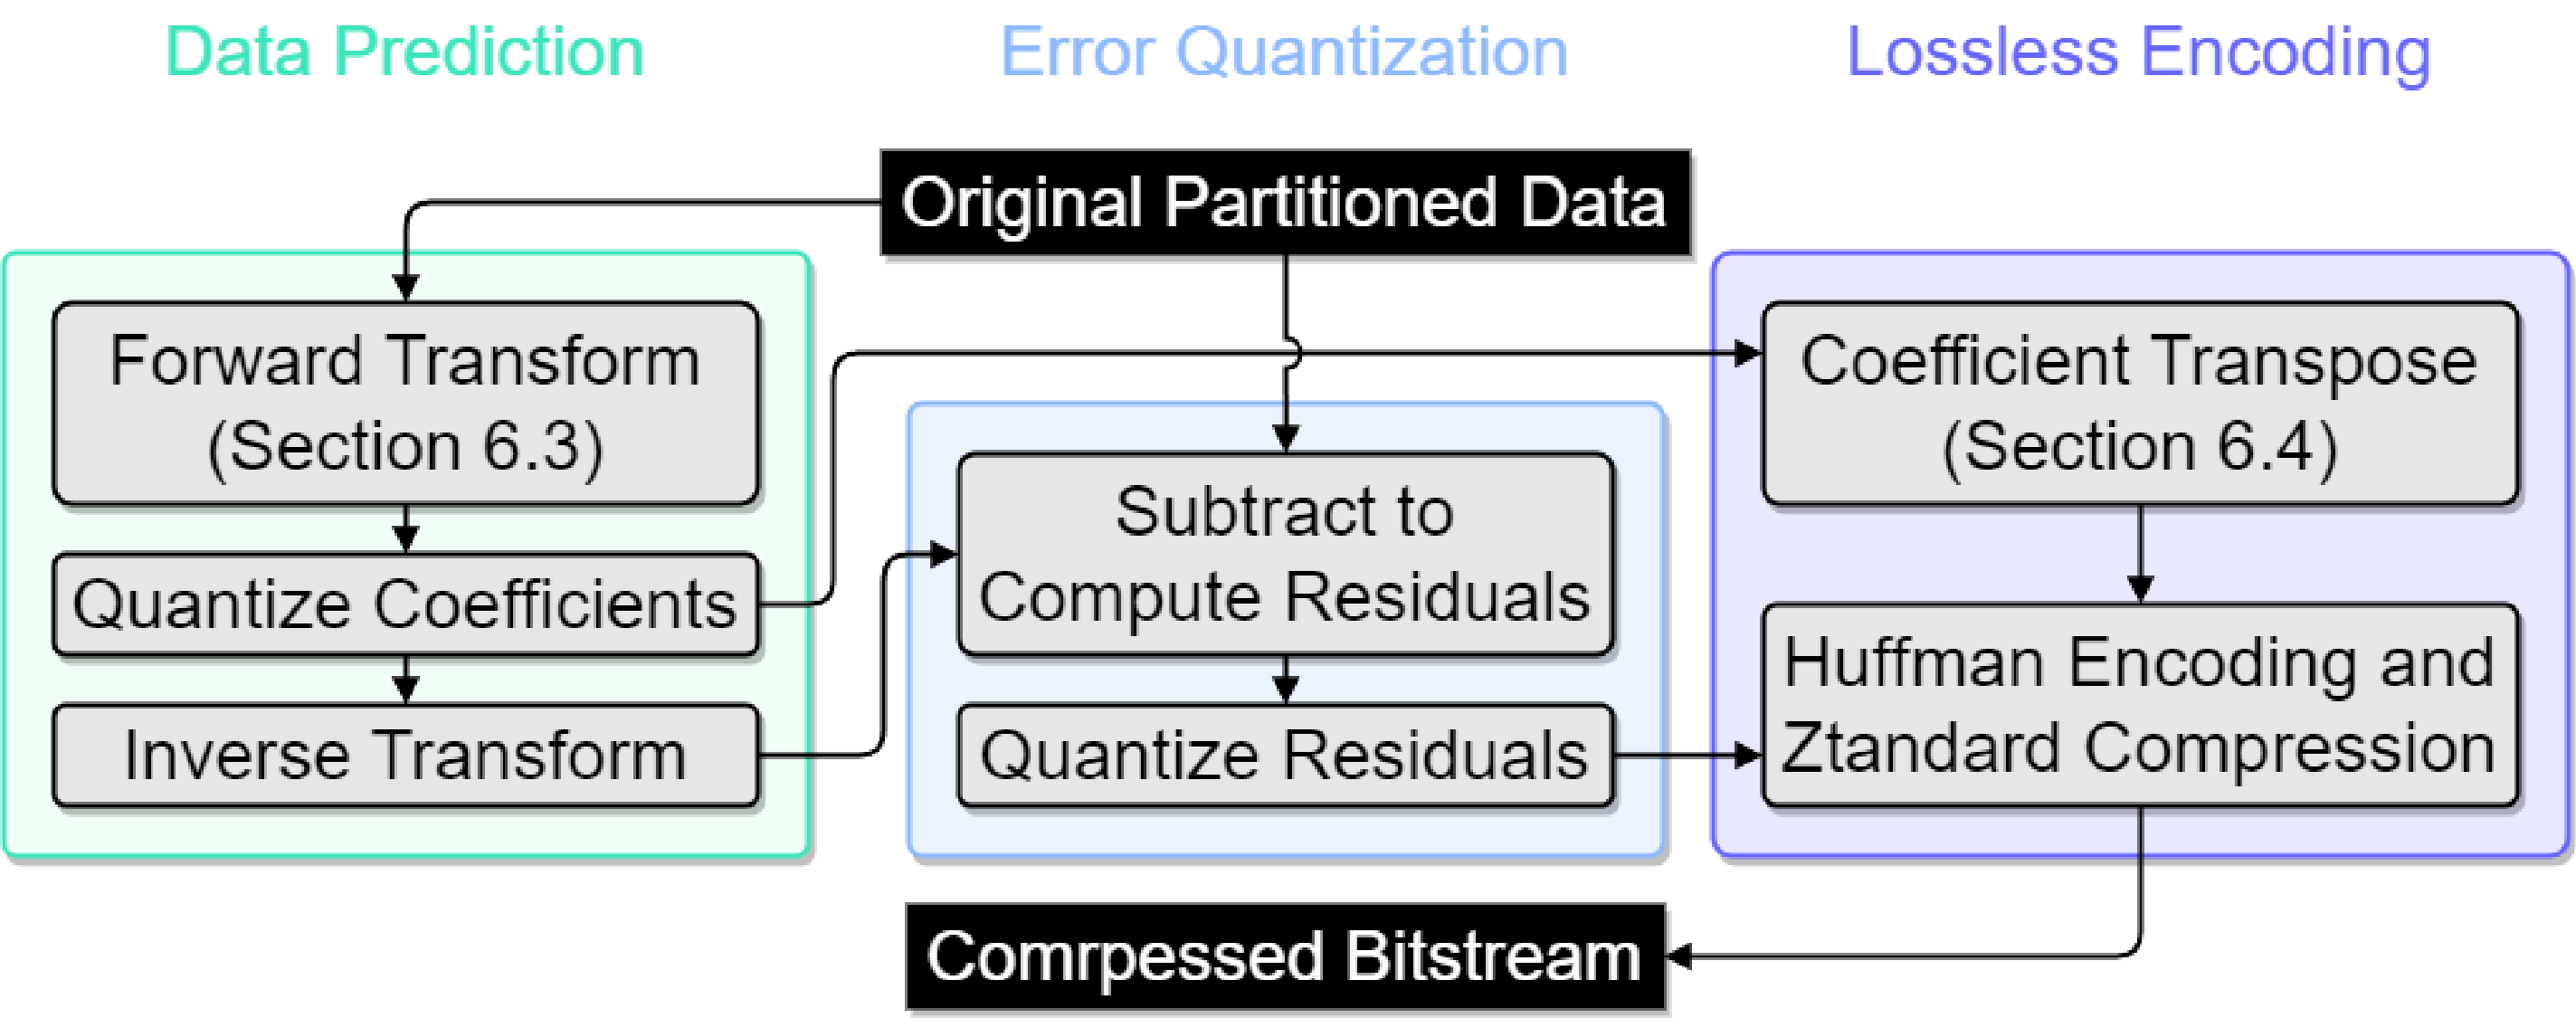
\includegraphics[width=1\linewidth]{figs/6/mrcz diagram.pdf}
    \caption{Diagram of MRCZ Compression.}
    \label{fig:mrcz_diagram}
\end{figure}

Figure~\ref{fig:mrcz_diagram} illustrates the overall workflow of MRCZ. Similar to other SZ-family compressors, MRCZ consists of three main stages: data prediction, error-bounded quantization, and lossless encoding.

During data prediction, MRCZ applies a forward transform to each element, quantizes the resulting transform coefficients using a dedicated coefficient error bound, and then performs an inverse transform on the quantized coefficients to generate approximate predictions. The residuals between the original data and these predictions are subsequently quantized under the user-specified error bound. Consequently, in addition to the quantized residuals stored by conventional SZ-family compressors, MRCZ must also store the quantized transform coefficients required to reproduce the predictions during decompression.

The residual quantization and lossless encoding stages otherwise follow the standard SZ-family pipeline described in Section~\ref{sec:design overview:family}. Before lossless encoding, MRCZ additionally transposes the quantized coefficient layout to improve its compressibility, as discussed in Section~\ref{sec:mrcz:transpose}.

\subsection{Transform and Error Bound Selection}

In addition to the choice of transform, the coefficient error bound also has a significant impact on compression performance. A smaller coefficient error bound preserves the transform coefficients more accurately, but produces more finely quantized coefficient symbols that are generally less compressible. At the same time, the resulting predictions are more accurate, leading to smaller residuals that are easier to compress. If the coefficient error bound is excessively small, the prediction error after the inverse transform may remain below the user-specified error bound for most or even all data points. In this case, the available error budget is underutilized, resulting in higher reconstruction quality than required at the cost of a lower compression ratio.

\begin{figure}[htb]
    \centering
    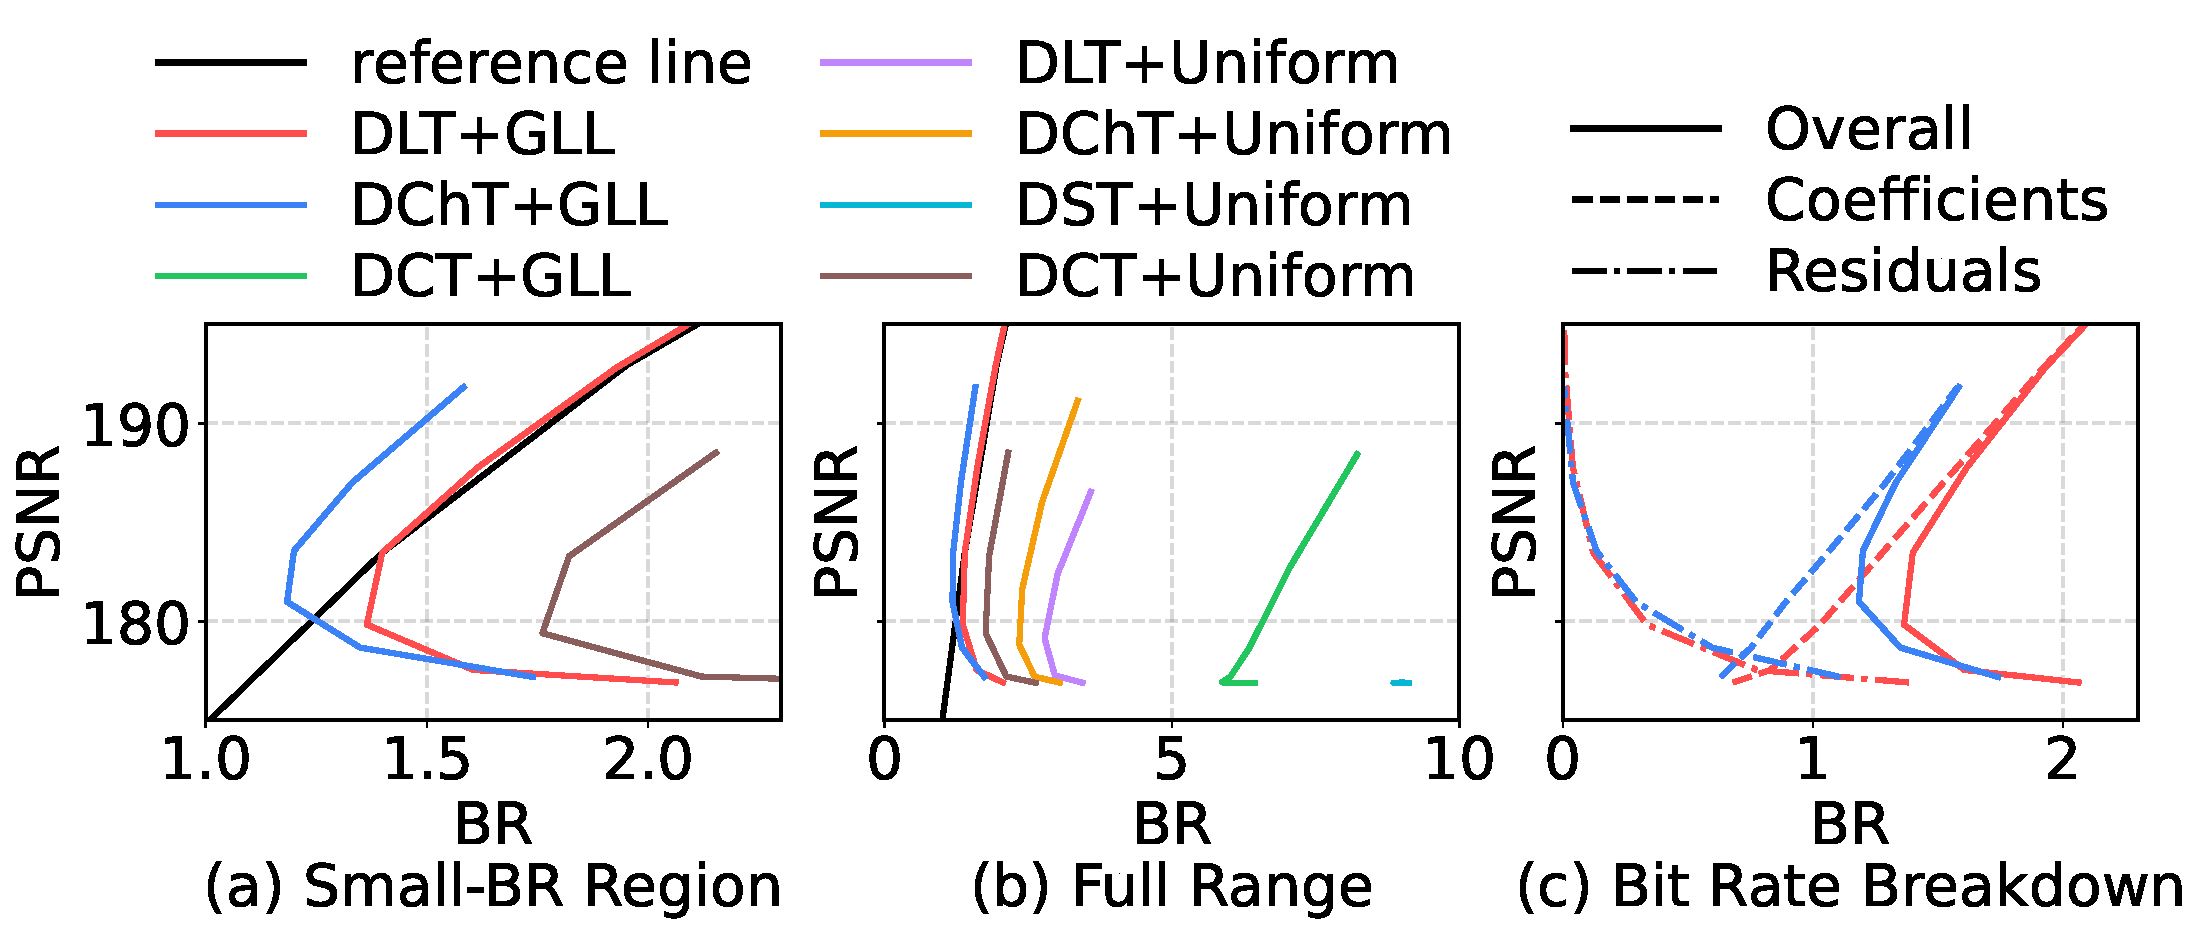
\includegraphics[width=1\linewidth]{figs/6/transform-comparison.pdf}
    \caption{Rate–Distortion Performance and Bit-Rate Breakdown of Different Transforms Across Error-Bound Configurations}
    \label{fig:transform}
\end{figure}

To study this trade-off, we use DLT as an example and define $k_{eb}=\frac{eb_{coeff}}{eb_{value}}$, where $eb_{coeff}$ is the coefficient error bound and $eb_{value}$ is the user-specified data error bound. We first fix $eb_{value}$ and vary $k_{eb}$, producing the red solid curve in Figure~\ref{fig:transform}(a). For reference, we also plot a conventional rate--distortion curve by fixing $k_{eb}$ and varying $eb_{value}$ (black solid curve). This reference curve characterizes the compressor performance under different user-specified error bounds. 

When $k_{eb}$ is too small, the red curve nearly overlaps the reference curve. In this regime, the compressor produces data with higher fidelity than required by the user, at the cost of a lower compression ratio. An appropriate value of $k_{eb}$ is therefore near the transition at which the red curve begins to deviate noticeably from the reference curve. For DLT, this transition occurs at approximately $k_{eb}=0.1$.

We next compare different transforms under the same user-specified data error bound. Figures~\ref{fig:transform}(a) and \ref{fig:transform}(b) present the rate--distortion curves for the evaluated transforms, obtained by varying $k_{eb}$, together with the black reference curve described above. We evaluate DLT, DCT, DST, and DChT using two node-location assumptions. In the figure legends, the ``GLL'' variants use the actual GLL node locations, whereas the ``Uniform'' variants treat the input values as samples on a uniformly spaced grid.

Among the evaluated transforms, DChT+GLL generally achieves the best rate--distortion performance. Portions of its curve lie to the left of the reference curve, indicating that it can achieve a lower bit rate, and equivalently a higher compression ratio, than the DLT-based reference configuration at comparable distortion levels. Overall, DChT+GLL improves the compression ratio by approximately 20\% over DLT+GLL at the same PSNR. For DChT+GLL, the corresponding transition occurs at approximately $k_{eb}=0.05$. Based on these results, we adopt DChT+GLL with $k_{eb}=0.05$ as the core transform configuration in MRCZ and refer to it simply as DChT hereafter.

To better understand the source of the performance difference between DChT and DLT, we separately compress the transform coefficients and the residuals produced by each transform. Figure~\ref{fig:transform}(c) shows the resulting rate--distortion curves for DChT and DLT on GLL nodes. The residual curves of the two transforms nearly overlap, indicating that their residuals have similar compressibility. In contrast, the coefficient curve of DChT lies consistently to the left of that of DLT, showing that the coefficients produced by DChT can be compressed at a lower bit rate for a comparable distortion level. Therefore, the overall rate--distortion advantage of DChT primarily comes from the improved compressibility of its transform coefficients rather than from differences in the residuals.

\subsection{Improving Local Regularity for Lossless Encoding}\label{sec:mrcz:transpose}

We further investigate whether the quantized transform coefficients can be made more compressible by improving their local regularity before lossless encoding. A related idea is used in QoZ2.0~\cite{liu2024high}, which applies lightweight spatial blocking based on the observation that neighboring data points often exhibit similar prediction errors. Such regularity may arise because higher-order information not fully captured by interpolation can still exhibit local spatial continuity. Grouping quantized prediction errors within small spatial blocks therefore creates more regular symbol sequences and improves the effectiveness of subsequent lossless encoding.

However, the source of regularity in MRCZ differs from that in interpolation-based compressors. Neighboring entries in an element's coefficient matrix represent different basis modes and have no direct notion of spatial proximity. MRCZ therefore exploits regularity across elements by grouping coefficients associated with the same basis mode. This effect is particularly pronounced for higher-order modes, whose coefficients are frequently quantized to zero across many elements.

Motivated by these observations, we transpose the coefficient layout from element-major order to mode-major order, grouping coefficients associated with the same basis mode across multiple elements. This layout places frequently zero-valued higher-order coefficients and statistically similar same-mode coefficients into more regular sequences, improving the effectiveness of lossless encoding and increasing the compression ratio by approximately 20\%.